\documentclass[journal]{IEEEtran}
\usepackage{cite}
\usepackage[cmex10]{amsmath}
\usepackage{graphicx}
\usepackage{amssymb}
\usepackage{booktabs}
\usepackage{algpseudocode,algorithm2e}
%\usepackage[justification=centering]{caption}
\hyphenation{op-tical net-works semi-conduc-tor}

\begin{document}
%
% paper title
% can use linebreaks \\ within to get better formatting as desired
% Do not put math or special symbols in the title.
\title{Active Learning Based Constrained Clustering For Speaker Diarization}
%
%
% author names and IEEE memberships
% note positions of commas and nonbreaking spaces ( ~ ) LaTeX will not break
% a structure at a ~ so this keeps an author's name from being broken across
% two lines.
% use \thanks{} to gain access to the first footnote area
% a separate \thanks must be used for each paragraph as LaTeX2e's \thanks
% was not built to handle multiple paragraphs
%

\author{Chengzhu~Yu,~\IEEEmembership{Student~Member,~IEEE,}
        and John~H.~L.~Hansen,~\IEEEmembership{Fellow,~IEEE}}% <-this % stops a space
%\thanks{M. Shell is with the Department
%of Electrical and Computer Engineering, Georgia Institute of Technology, Atlanta,
%GA, 30332 USA e-mail: (see http://www.michaelshell.org/contact.html).}% <-this % stops a space
%\thanks{J. Doe and J. Doe are with Anonymous University.}% <-this % stops a space
%\thanks{Manuscript received April 19, 2005; revised December 27, 2012.}}

% note the % following the last \IEEEmembership and also \thanks - 
% these prevent an unwanted space from occurring between the last author name
% and the end of the author line. i.e., if you had this:
% 
% \author{....lastname \thanks{...} \thanks{...} }
%                     ^------------^------------^----Do not want these spaces!
%
% a space would be appended to the last name and could cause every name on that
% line to be shifted left slightly. This is one of those "LaTeX things". For
% instance, "\textbf{A} \textbf{B}" will typeset as "A B" not "AB". To get
% "AB" then you have to do: "\textbf{A}\textbf{B}"
% \thanks is no different in this regard, so shield the last } of each \thanks
% that ends a line with a % and do not let a space in before the next \thanks.
% Spaces after \IEEEmembership other than the last one are OK (and needed) as
% you are supposed to have spaces between the names. For what it is worth,
% this is a minor point as most people would not even notice if the said evil
% space somehow managed to creep in.



% The paper headers
\markboth{IEEE/ACM TRANSACTIONS ON AUDIO, SPEECH, AND LANGUAGE PROCESSING} %
{Shell \MakeLowercase{\textit{et al.}}: Bare Demo of IEEEtran.cls for Journals}
% The only time the second header will appear is for the odd numbered pages
% after the title page when using the twoside option.
% 
% *** Note that you probably will NOT want to include the author's ***
% *** name in the headers of peer review papers.                   ***
% You can use \ifCLASSOPTIONpeerreview for conditional compilation here if
% you desire.

% If you want to put a publisher's ID mark on the page you can do it like
% this:
%\IEEEpubid{0000--0000/00\$00.00~\copyright~2012 IEEE}
% Remember, if you use this you must call \IEEEpubidadjcol in the second
% column for its text to clear the IEEEpubid mark.

% use for special paper notices
%\IEEEspecialpapernotice{(Invited Paper)}

% make the title area
\maketitle

% As a general rule, do not put math, special symbols or citations
% in the abstract or keywords.
\begin{abstract}
Most speaker diarization researches focus on unsupervised scenarios, where no human supervision is available. However, in many real-world applications, certain amount of human input could be engaged, especially when minimal human supervision brings significant performance improvement. In this paper, we propose an active learning based bottom-up speaker clustering algorithm to effectively improve speaker diarization performance with limited human input. Specifically, proposed active learning based speaker clustering has two different stages: \textit{explore} and \textit{constrained clustering}.
The purpose of \textit{explore} stage is to quickly discover at least one sample for each speaker for boosting the speaker clustering process with reliable initial speaker clusters. After discovering all or majority of involved speakers during \textit{explore} stage, the \textit{constrained clustering} is performed. The \textit{constrained clustering} is similar to traditional bottom-up clustering process with an important difference that the speaker clusters created during \textit{explore} stage is restricted to merge with each other during clustering. The \textit{constrained clustering} continues until only the clusters generated from \textit{explore} stage are left. 

While above active learning based speaker clustering algorithm could rapidly reduce the diarization error rate (DER) with relatively small amount of human input, its performance saturates as human input increases. To overcome this limitation, we propose an active learning based cluster reassignment algorithm to further improve the diarization performance. The active learning based cluster reassignment algorithm, is to select the clustered segments that accounted for the largest expected speaker error (ESE) for human evaluation and reassignment. 

We evaluate above two active learning algorithms on our recently created Apollo Mission Control Center (Apollo-MCC) dataset as well as AMI meeting corpus. The results indicate that proposed active learning algorithms could effectively utilize human input to improve speaker diarization performance.

%While the concept of \textit{explore} and \textit{consolidate} are borrowed from the area of data mining, a substantial changes are made here for the application of speaker diarization. 
%The main purpose of \textit{explore} and \textit{consolidate} stages in proposed algorithm, is to  To achieve this, we uses farthest first query search (FFQS) with active learning to quickly discover at least one sample for each speaker during \textit{explore} phase, and employ nearest neighbor query search (NNQS) during \textit{consolidate} phase to ensure reliable instances for each discovered speaker cluster. After \textit{explore} and \textit{consolidate} phases, the standard bottom-up clustering is performed with a constraint that the clusters discovered during \textit{explore} phases are not merged with each other.
Finally, 
     
\end{abstract}

% Note that keywords are not normally used for peerreview papers.
\begin{IEEEkeywords}
Speaker diarization, active learning, bottom-up clustering
\end{IEEEkeywords}

% For peer review papers, you can put extra information on the cover
% page as needed:
% \ifCLASSOPTIONpeerreview
% \begin{center} \bfseries EDICS Category: 3-BBND \end{center}
% \fi
%
% For peerreview papers, this IEEEtran command inserts a page break and
% creates the second title. It will be ignored for other modes.
\IEEEpeerreviewmaketitle

\section{Introduction}
\label{intro}
Speaker diarization is the process of automatically detecting \textit{who spoke when }in an audio sequence. With increasing amount of audio resources, speaker diarization becomes an important technology in many applications such as information retrieval, metadata extractions, meeting annotations, and conversation analysis. Recent developments for speaker diarization algorithms have been largely driven by Rich Transcription (RT), where speaker diarization plays a role to provide speaker index and other information to achieve improved speech-to-text transcriptions.

As a sequential process, speaker diarization normally involves several components such as voice activity detection, speaker change detection (segmentation), clustering, and re-segmentation. Among theses components, the core part of speaker diarization is clustering, where it separate segments from different audio sources such as speaker, music, and noise, and group them together. Due to its significance, various speaker clustering solutions have been proposed. Theses include but not limited to bottom-up approach, also known as agglomerative hierarchical clustering (AHC), top-down approach, and recently proposed global optimization approaches. 

Bottom-up clustering is in general the most popular strategy among various clustering solutions. It starts by treating each individual segments, obtained in the segmentation stage, as separate clusters, and iteratively merging the closest two clusters until a specified stopping criteria is satisfied. While not as popular as its counterpart, top-down approach has also been widely applied and some studies have reported that it could achieve comparable result with bottom-up clustering [Evans, 2012]. Different from bottom-up based approach, top-down clustering starts from modeling the entire audio as single model and iteratively splitting the model into sub clusters until a stopping criteria is met. Despite their differences, both bottom-up and top-down based approach are iterative process and has the drawback of error propagation. A recently proposed clustering algorithm, Interger Linear Programming (ILP), attempts to overcome this drawback by finding the cluster assignments that jointly minimizing the number of assigned clusters as well as within-cluster dispersion. While the ILP could avoid the drawbacks of error propagation, it has to start with initial clusters containing sufficient samples for estimating its characteristic (e.g., i-vector). Therefore, ILP is mostly performed after bottom-up clustering.

Along with the development in speaker clustering, the distances metric used for measuring wheter two segments belong to same class, has also made significant improvement from original Bayesian informative criteria (BIC), generalized log-likelihood ration (GLR), Kullback-Leibler (KL) divergence, to recent i-vector based distances such as cosine distance score (CDS) as well as probablistic linear discriminant analysis (PLDA) based distance. Other alternative distance metrics, such as these based on information theoretic framework are also proposed and showed competitive results. 

Despite the success of recent improvement on speaker clustering algorithms, distance computations, as well as other non-trivial components, speaker diarization still remains as a challenging tasks in many real-word applications, especially where the audio quality is suboptimal or the speech communications comprises large proportions of fast speaker turns and short homogeneous speech segments. For example, diarization of telephone conversations are notably more challenging compared with broadcast news diarization, as well as meeting room diarization. 

Due to the limitation within current speaker diarization systems using exclusively audio/speech information, a number of recent studies have proposed to exploit auxilary informations for improved speaker diarization performance. For example, the linguist information such as speaker name occurring patterns are extracted from the speech transcripts to provide additional information during speaker clustering. The speech transcript could be obtained from manual transcript as well as automatic speech recognition system. Another important supplementary information that presents in many speaker diarization applications is the visual information. The audio-visual speaker diarization has also been studied. However, these auxilary information are obtainable only in certain scenarios and not applicable to broad category of speaker diarization applications.

In this study, we propose an active learning based, bottom-up speaker clustering algorithm that effectively utilize human input to improve speaker diarization performance. Our proposed algorithm is based on the assumption that human input could be engaged during speaker diarization process in certain applications. This scenario is especially plausible if small amount of human engagement could brings significant performance improvements. Another assumption we made in this paper is that, human is better than machine for recognizing whether a given segment pair is from the same speaker or not. This assumption is based on the results from previous studies that while current speaker recognition systems shows competitive performance as human in clean speech condition, in adverse conditions human significantly outperform machine. Besides, many audio streams for speaker diarization applications contain higher level information such as video, spoken names, and contextual informations that could effectively employed by human for performing speaker recognition.

While human can effective determine whether two segments belong to the same speaker or not, tagging the ground truth speaker labels of audio segments containing large number of participants is significantly more difficult task. This is due to the limitations of human ear in remembering voices from different speakers. The comprehensive labeling of speaker index for these tasks need to be achieved by answering a series of queries: a \textit{yes or no} type of questions asking whether a given segments pair belongs to the same speaker or not. The total number of queries for obtaining perfect clustering results requires human to evaluate $\dfrac{N(N-1)}{2}$ queries, where N indicates the number of speech segments. Therefore, an effective active query selection strategy is necessary in order to effectively employ human input to boosting the speaker diarization performance. 

To effectively employ human input, we first need to identify which part of speaker clustering components have largest effect on final speaker diarization performance. A recent study by [Simon King] has evaluated several key components of speaker diarization and concluded that initial speaker models with pure and reliably labeled data could lead to significant improvement to the overall speaker diarization performance.  Motivated by the above study, we designed our active learning algorithm to quickly discover all or most of the speakers in audio stream in the \textit{explore} phase, and initiate speaker clustering using reliable initial speaker models. We also propose to perform bottom up clustering with \textit{constrained clustering} after \textit{explore} stage, where initial clusters from \textit{explore} stages, will not be merged together. This proposed algorithm is a way of turning unsupervised speaker clustering problems into a slightly supervised close-set speaker identification tasks, with speaker models updates at each iteration.

In addition to active learning for improved speaker clustering process, we also investigate the use of active learning for cluster reassignment after finishing clustering process. The objective of proposed active learning based cluster reassignment, is to actively select certain speech segments from clustered results for human evaluation and reassignment. The essence of active learning based cluster reassignment, is to effectively locate most informative segments. In this study, we achieve this by selecting speech segments with largest expected speaker error as candidates for human evaluation.

To summary, in this study, we investigate the use of active learning for bottom-up speaker clustering. We proposed two different strategies where active learning are employed for robust initial cluster estimation and post clustering reassignment, respectively. The remainder of paper is organized as follows. In Sec.\ref{rw}, we will introduce previous studies on active learning for bottom-up clustering. In Sec.\ref{bs}, we will give brief overview of the bottom-up speaker clustering based on i-vector cosine distance score (CDS), which serve as our baseline system.   

\begin{figure*}
	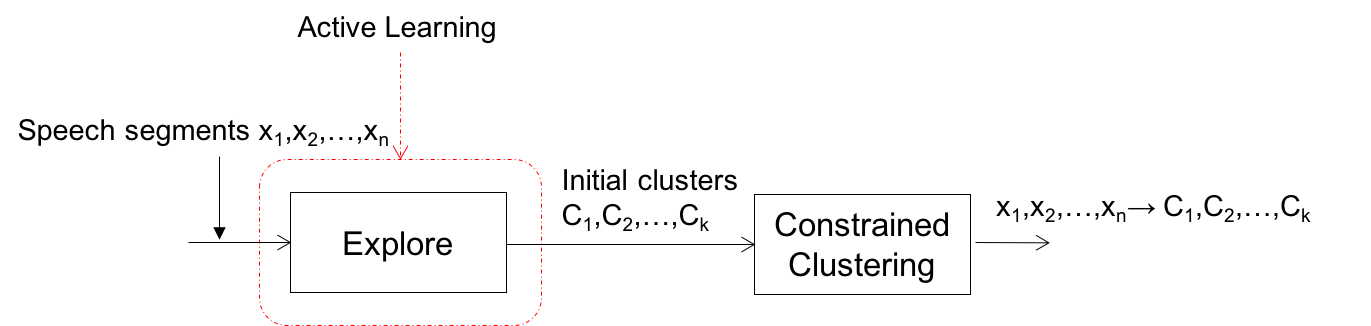
\includegraphics[width=\linewidth]{figs/flow5}
	\caption{Diagram of active learning based bottom-up speaker clustering. The red dotted block is active learning component where human involves.}
	\label{fig:flow1}
\end{figure*}

\section{Related Work}
\label{rw}
Active learning based constrained clustering has been extensively studied for image clustering tasks and in broader area of data mining. A number of algorithms have been proposed to use active learning for clustering unlabeled data with human in the loop. The key idea behind these algorithms is to actively select pairs of data for human to provide answer in a form of yes or no. 
Most of the algorithms proposed in these studies, are targeting k-means clustering, and normally composed of two stage: \textit{explore} and \textit{consolidate}. The purpose \textit{explore} phase is to find the centroids of different clusters, and the aim of consolidate stage is to locate most informative data pair for human labeling. While the fundamental problem of these studies is much similar to the problem we have in speaker diarization, active learning for speaker diarization is more challenging task in general due to the reasons below. Firstly, the bottom-up clustering in speaker diarization requires to iteratively update the cluster statistics at each iteration. Therefore, the decisions in current iteration has a reliance on previous iteration, and it is difficult to quantify the importance of each segment pair during clustering. Another important difference is that, the total number of cluster numbers in speaker diarization are unknown most of time. Due to these differences, the direct replication of active learning algorithms developed in these studies, is not viable.

On the other hand, only a limited number of studies in the area of speaker recognition and diarization, has investigates the use of active learning for speaker diarization tasks. For example, the study by [Shum] has investigate to use active learning to obtain background speaker labels from unlabeled data for training PLDA system. While the study by [Shum] bears similarity with this paper, the ultimate goal of [Shum] is to locate reliable samples sufficient enough to train PLDA system, rather than clustering entire dataset as in speaker diairization task. Another study, that employ active learning for speaker diarization is by [Mateusz]. The criteria of active selection for human labeling in [Mateusz] is simply based on the length of speech segment, which will not work in many speaker diarization task where the variance of segment length is small.

\section{Baseline System}
\label{bs}
The baseline speaker diarization system used in this study, is a bottom-up speaker clustering algorithm with i-vector cosine distances score (CDS) as distance metric. In this section, we will give a brief discussion about i-vector extraction, CDS and bottom-up speaker clustering. 

\subsection{i-vector extraction}
In i-vector extraction framework, speaker and channel dependent GMM supervector is modeled as follows:
\begin{equation}
\begin{aligned}
& M=m+Tw,
\label{mmtw}
\end{aligned}
\end{equation}
where $m$ is the supervector obtained from the universal background model (UBM), 
$T$ is the low rank total variability matrix representing the basis of reduced total variability space, 
and $w$ is the low rank factor loadings referred to as i-vectors. 

The estimation of the total variability matrix $T$ employs expectation maximization (EM) method as described in \cite{kenny2005eigenvoice}. 
After training the total variability matrix, 
the i-Vector of given speech utterance is extracted as the conditional expectation of i-Vector distribution given observation features.
\begin{equation}
\begin{aligned}
&w_{s}^{\ast}=E[P(w_{s}|X_{s})],
\label{eq:ws}
\end{aligned}
\end{equation}
where $w_{s}^{\ast}$ is the i-Vector of the given speech utterance $s$, 
$X_{s}$ is the clean observation features, 
$P(w_{s}|X_{s})$ is the conditional distribution of the i-Vector given observation features, 
and $E[\cdot]$ indicates the expectation. 
Finally, the i-Vector of the given speech utterance can be represented using the Baum-Welch zeroth ($N_s$) and centralized first ($F_s$) order statistics,
\begin{equation}
\begin{aligned}
&w_{s}^{\ast}=(T'N_{s}\Sigma^{-1}T+I)^{-1}T\Sigma^{-1}F_{s},
\label{ws2}
\end{aligned}
\end{equation}
where $\Sigma$ is the covariance matrix obtained from UBM model and $I$ is the identity matrix.

\subsection{Cosine Distance Score}
Comparison of  i-vectors from two different segments, could be successfully achieved with simple cosine similarity. The cosine distance score between two vectors could be expressed as follow:
\begin{equation}
\begin{aligned}
& score (w_i, w_j) = \dfrac{w^T_i \cdot w_j}{\rvert\rvert{w_i}\rvert\rvert \cdot \rvert\rvert{w_j}\rvert\rvert}.
\label{ws2}
\end{aligned}
\end{equation}
Note that, the score of cosine distance ranges between [-1, 1]. The higher the number towards 1, the more similarity exist between two vectors. The cosine distance score has been a popular metric for speaker recognition and verification in i-vector space.
 
\subsection{Bottom-up Speaker Clustering}
Bottom-up clustering, also known as hierarchical agglomerative clustering (HAC), has been the most popular speaker clustering algorithm used for speaker diarization. It typically starts by treating all homogeneous speech segments as a separate cluster, and iteratively merge two closest clusters. In our study, for each iteration, we find two segments that has the highest cosine similarity, and merge them into a single cluster. After each iteration, i-vectors are extracted from updated clusters and normalized to have zero mean. We continue the iterations until the CDS of two closest cluster reaches specified stopping criteria. 

\section{Active Learning based Speaker Clustering}
Due to the error propagation characteristics of bottom-up speaker clustering, having good initial cluster model, has significant impact on final speaker diarization performance. In this section, we will give a detailed description of our proposed active learning strategy for bottom-up speaker clustering. As mentioned in introduction, the proposed algorithm has two clustering components: \textit{explore} and \textit{constrained clustering} as in the Figure.~\ref{fig:flow1}.

\begin{figure*}
	\centering
	
\includegraphics[width=\linewidth]{figs/flow6}
	\caption{Diagram of active learning based bottom-up speaker clustering. The red dotted block is active learning component where human involves.}
	\label{fig:flow2}
\end{figure*}

\subsection{Explore}
The purpose of \textit{explore} phase, is to quickly discover all speaker clusters within the audio streams, finding at least one speech segment for each speaker cluster. To achieve this, we use the farthest first query search (FFQS) proposed by [Basu]. With FFQS, a speech segment is randomly selected from all speech segments to be used as seed segment. The selected speech segment is then used to initialize the first cluster. After creating the first speaker cluster, the next segment is selected which is farthest from existing clusters. The chosen segment is then provided for human to provide expert opinion. If the chosen segment belongs to existing clusters after pairwise comparison, the new segment is merged to the corresponding cluster. Otherwise, a new cluster is created from the selected segment. Note that, in order to decided if a given speech segment belongs to a target cluster or not, we compose a query pair using the segment in question and the longest segment within the target cluster. If the answer returns by human expert is true, then the segment belongs to the target cluster, and vice versa. The FFQS process continues until the pairwise comparison operations reached specified maximum number specified by user. The details of \textit{explore} phase is detailed in Algorithm.~\ref{a1}.  

\begin{figure*}[t]
\centering
	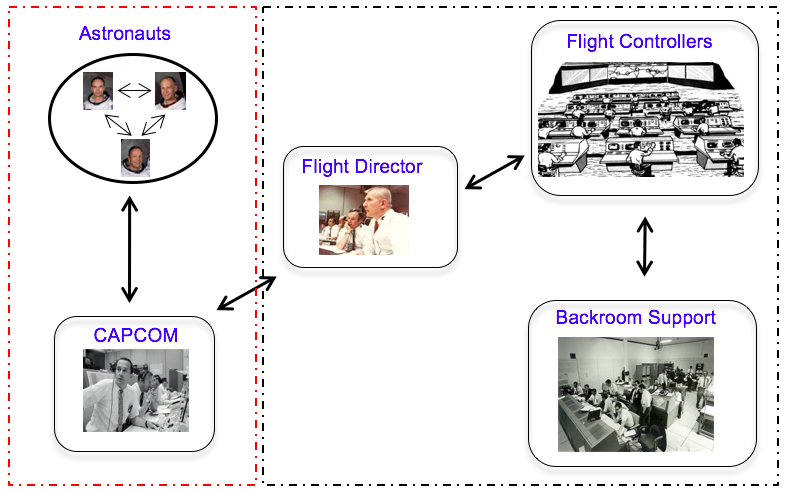
\includegraphics[width=0.75\linewidth]{figs/comm5}
	\caption{Apollo Mission Control Center (MCC) communication overview. The elements inside red dotted blocks are space-to-ground communications, including astronauts voice from space. The elements inside black dotted blocks are ground communications between hundreds of flight controllers and their 'backroom' supports. }
	\label{fig:comm}
\end{figure*} 
\begin{algorithm}
	\KwData{Set of speech segments $X = {\{x_i\}}_{i=1}^n$, acess to the answers of pairwise queries, maximum number queries $Q$ user specified. }
	\KwResult{$C_{k=1}^{k}$ initialized clusters}
	Start from null cluster $C= \{\}$\;
	Select a segment $x$ at random, and create the first cluster as $C_1 = \{x_i\}$, $\lambda \leftarrow 1$\; 
	\While{maximum queries not reached, $\lambda < Q$}{
		Find speech segment $x_{\lambda}$ farthest from existing clusters in $C$, based on i-vector cosine similarity scores.\;
		\eIf{$x_{\lambda}$ belongs to any clusters in $C$}{
			Add speech segment $x_{\lambda}$ to cluster matching cluster
		}{
			Create new cluster $C_k$ with speech segment $x_{\lambda}$\;
		}
		Increase $\lambda$, for each query access. 	
	}
	\caption{FFQS with random seed during \textit{explore} phase.}
	\label{a1}
\end{algorithm}
 
While the above algorithms could effectively explore the speaker clusters in the audio streams, its performance varies a lot depending on which seed segment is selected. This problem is due to the randomness during initial seed selection. The previous studies in k-means clustering has revealed that, the initial seed data should be closer to actual centroids in order to achieve favorable clustering results. Motivated by this, we first performed a fully unsupervised bottom-up clustering on the entire speech segments, and taking the centroid segment of each cluster as initial seeds to start FFQS algorithm during \textit{explore} phase.

\subsection{Constrained Merging}
After initial \textit{explore} phase, the standard bottom-up clustering is performed with two important exceptions. First, the clusters $C_{k=1}^{K}$ created during \textit{explore} stage, are restricted to not merge with each other. Second, the stopping distance threshold during bottom-up clustering is no longer necessary, as we have assumed all involved speakers are discovered during \textit{explore} phase. The bottom-up clustering will continues until only $C_{k=1}^{k}$ clusters remain.

\section{Active Learning Based Cluster Reassignment}
In previous section, we propose an active learning based algorithm to obtain better initial speaker models. Alternatively, human input could be involved after clustering finishes, to evaluate and fix incorrectly labeled speech segments. This is quite similar to the use of active learning for automatic speech recognition (ASR), where the sentence with less confidence is passed to human for corrections. However, the same algorithm used for ASR could not be directly applied in speaker diarization for several reasons. First, the confidence measure used for ASR is not appropriate for speaker diarization. Second, even though the potential erroneous segments are identified, the evaluation and reassignment process of these segments are much different.

The proposed active learning based cluster reassignment has three major components as in Fig.~\ref{fig:flow2}. 

\subsection{Candidates selection}
The cluster reassignment algorithm starts with selecting the candidate speech segments for human expert to review later. In order to effectively select most informative segments, we ranks all speech segments in terms of expected speaker error (ESE). In other words, we will select speech segments that will produce largest expected speaker error reduction. 
In this study, we compute the expected speaker error for each speech segment as below. 
\begin{equation}
\begin{aligned}
E(x_j) =& P(x_j | C_j) \cdot J_{x_j \in C_j} \\
&+ (1 - P(x_j | C_j)) \cdot J_{x_j \notin C_j}
\label{expect}
\end{aligned}
\end{equation}

where $x_j$ indicates $j$th speech segment, $C_j$ is the cluster assigned to speech segment $x_j$, $P(x_j|C_j)$ is the probability of segment $x_j$ belongs to cluster $c_j$, $J_{x_j \in C_j} $ is the speaker error if $x_j$ belongs to cluster $C_j$, and $J_{x_j \notin C_j}$ is the speaker error if $x_j$ not belongs to cluster $C_j$. We could also write that
\begin{equation}
\begin{aligned}
&J_{x_j \in C_j} = 0 \\
&J_{x_j \notin C_j} = \dfrac{d_j}{\sum_{i=1}^{n} d_i}
\label{jj}
\end{aligned}
\end{equation} 
where $d_j$ is the length of speech segment $x_j$, and $\sum_{i=1}^{n} d_i$ is total length sum of all speech segments of the testing audio stream.

We compute $P(x_j|C_j)$ by modeling a multivariate Gaussian distribution for each $C_{k=1}^{k}$ using i-vectors of all the segments of given cluster. We normalize the probability to sum to one.
\begin{equation}
\begin{aligned}
&  \sum_{i=1}^{k} P(x_j|C_i) = 1;
\label{jj}
\end{aligned}
\end{equation}
 
\subsection{Evaluation}
After selecting the candidate segments, human expert will determine whether the given segment belongs to its assigned cluster. The process of employing human input to decide whether a segment belongs to a cluster, is more difficult than the strategy we used in \textit{explore} phase of previous section. We could not simply select a single longest segment in the cluster, and compose query pair with the segment in question. This is due to the fact that chosen longest segment of the cluster, could be an incorrect assignment. Therefore, we employ a majority voting based segment cluster evaluation strategy. Under this strategy, the segment in question is paired with each segments within assigned cluster, resulting in multiple query pairs. If majority answers of these pairs are true (two segments belong to the same cluster), we will make a decision that the given speech segment has correct cluster assignment, and vice versa. 

While the above strategy is robust for evaluating whether a given segment belongs to target cluster, it involves significant number of query pairs for human evaluation. One heuristic that we used in our study is to set a maximum query number limit $V$ for each segment evaluation. We rank speech segments assigned to target cluster by its confidence $P(x|c)$, and select top $V$ confident segments as representatives of that cluster. These selected representative segments will be paired with test segment for majority voting based evaluation. 

\subsection{Correction}
After detecting segments with incorrect cluster assignment in \textit{evaluation} stage, we need to find the correct cluster designation for these segments. To achieve this, we employ N-best cluster evaluation.
We find the $N$ most possible cluster candidates for given segment by ranking the i-vector Gaussian posterior probabilities $P(x|C)$. The human expert will evaluate in order whether the given segment belongs to any of these N clusters, using the majority voting scheme as in the \textit{evaluation} stage. 

\section{Test Data}
We performs experiments on two different speech database: Apollo Mission Control Center (MCC) audio  corpus and AMI meeting corpus. 

\begin{table}[t]
	\centering
	\caption{Synopsis of Apollo-MCC audio dataset.}
	\label{syn}
	\begin{tabular}{|c|c|c|c|}
		\hline
		Session Name & Speech (seconds) & Speech Segments & Participants \\ \hline
		FD-01        & 252              & 161             & 9            \\ \hline
		FD-02        & 314              & 152             & 9            \\ \hline
		FD-03        & 123              & 63              & 10           \\ \hline
		FD-04        & 651              & 358             & 13           \\ \hline
		FD-05        & 457              & 226             & 14           \\ \hline
		FD-06        & 979              & 531             & 12           \\ \hline
		FD-07        & 394              & 267             & 13           \\ \hline
		FD-08        & 486              & 340             & 15           \\ \hline
		FD-09        & 217              & 126             & 13           \\ \hline
		FD-10        & 964              & 713             & 13           \\ \hline
		EECOM-01     & 1206             & 585             & 20           \\ \hline
		EECOM-02     & 563              & 252             & 20           \\ \hline
		EECOM-03     & 1014             & 471             & 31           \\ \hline
		EECOM-04     & 808              & 384             & 20           \\ \hline
		EECOM-05     & 812              & 357             & 26           \\ \hline
		EECOM-06     & 475              & 270             & 23           \\ \hline
		EECOM-07     & 553              & 337             & 21           \\ \hline
		EECOM-08     & 411              & 261             & 19           \\ \hline
		EECOM-09     & 744              & 430             & 31           \\ \hline
		GNC-01       & 859              & 270             & 17           \\ \hline
		GNC-02       & 735              & 346             & 21           \\ \hline
		GNC-03       & 653              & 291             & 25           \\ \hline
		GNC-04       & 1347             & 494             & 20           \\ \hline
		GNC-05       & 798              & 440             & 21           \\ \hline
		GNC-06       & 985              & 456             & 24           \\ \hline
		GNC-07       & 829              & 481             & 24           \\ \hline
		GNC-08       & 764              & 435             & 29           \\ \hline
		GNC-09       & 1728             & 995             & 29           \\ \hline
	\end{tabular}
\end{table}
\begin{table}[]
	\centering
	\caption{Synopsis of 12 meeting subset of AMI corpus.}
	\label{ami}
	\begin{tabular}{|c|c|c|c|}
		\hline
		Session Name & Speech (seconds) & Speech Segments & Participants \\ \hline
		IS1000a & 809 & 309 & 3 \\ \hline
		IS1001a & 165 & 102 & 3 \\ \hline
		IS1001b & 912 & 315 & 3 \\ \hline
		IS1001c & 591 & 212 & 3 \\ \hline
		IS1003b & 868 & 342 & 3 \\ \hline
		IS1003d & 661 & 441 & 3 \\ \hline
		IS1006b & 1288 & 315 & 3 \\ \hline
		IS1006d & 698 & 436 & 3 \\ \hline
		IS1008a & 346 & 77 & 3 \\ \hline
		IS1008b & 920 & 137 & 3 \\ \hline
		IS1008c & 926 & 236 & 3 \\ \hline
		IS1008c & 729 & 230 & 3 \\ \hline
	\end{tabular}
\end{table}

\subsection{Apollo-MCC Audio Corpus}
\label{apollo}
During the NASA Apollo mission, all communications between astronauts, flight controllers inside mission control center (MCC), and their backroom support teams are continuously recorded using a 30-track analog reel-to-reel recording machine. During each mission, a total of 60 audio channels are simultaneously recorded including the voices from more than hundred of different participants of the mission. The University of Texas at Dallas (UTD), University of Maryland College Park (UMD), and Johnson Space Center(JSC) has combined the effort to digitize this data resource and have generated up to 19,000 hours of audio data from various missions of both Apollo and Gemini missions. Those mission audio records the full detail of the Apollo communication, therefore extremely attractive for learning human-to-human communications, group interaction, as well as developing robust speech system. 

\begin{figure}[t]
	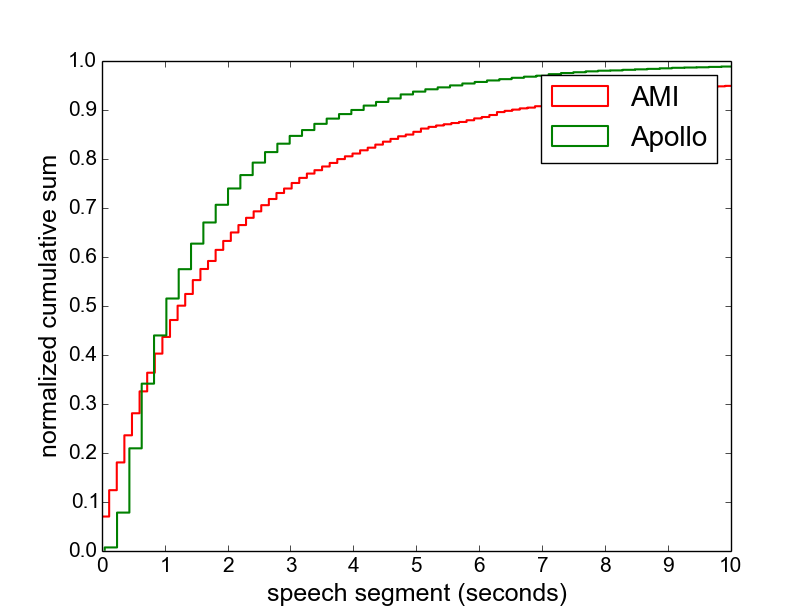
\includegraphics[width=\linewidth]{figs/lens}
	\caption{Cumulative histogram as a function of speech segments length for Apollo-MCC audio corpus and AMI meeting corpus.}
	\label{fig:cumu}
\end{figure}

Moreover, as the speech community (including us) rely on labeled audio data to perform scientific research as well as algorithmic development, we have prepared a 'Task Specific' corpus based on a subset of Apollo-11 audio recordings. We performed our experiment on this subset of Apollo-11 audio recordings which includes 3 synchronized channels: Flight director (FD) loop, Electrical, Environmental and Consumables Manager (EECOM) loop, and Guidance, Navigation, and Controls Systems Engineer(GNC) loop.  Each of these audio recording spanning approximately 10-hours before, and after lunar landing. This initial 28 hours task corpus has been transcribed to have speaker labels by well-trained speech science students from UTDallas \footnote{The task corpus will be released to the speech community for research and algorithmic development.}.

The audios in Apollo-MCC audio corpus includes two types of communication: space-to-ground communications between astronauts and Capsule Communicator (CAPCOM) in the ground, and ground communications between hundreds of flight controllers and "backroom" supports, see Figure.~\ref{fig:comm}. Most of these audios are recorded with close-talking microphones and are in general good audio quality. The audios from astronauts transmitted through Earth's dedicated telephone channels to Houston from ground stations where the signal was received. The flight directors as well as their "backroom" supports voice are recorded through intercom circuit called "loops". Each flight director has their own loops, which records the entire communication within that channel. The Apollo-MCC audio corpus is separated into 28 individual audio streams, with each of them containing 60 minutes of audios. The summary information about these audio files, including the length of pure speech after removing silence, number of homogeneous speech segments, and the total number of participants in each audio stream, are listed in Table.~\ref{syn}.

The voice communication style withing Apollo mission control center is much different from both traditional meeting corpus, including many short speech segments which was intended to improve communication efficiency. The Fig.~\ref{fig:cumu} shows cumulative histogram as a function of speech segments length. It can be observed that the Apollo-MCC audio dataset has larger proportions of audios are composed of short speech segments (less than 3sec) compared to AMI meeting data. Another major challenges in Apollo-MCC audio dataset is the number large number of participants as shown in Table.~\ref{syn}. Overall, diarization of Apollo-MCC audio dataset a very realistic and challenging task.

\subsection{AMI Meeting Dataset}
We also evaluate proposed algorithms in the popular 12-meeting subset of Augmented MultiParty Interaction (AMI) corpus. This is approximately 5.4 hours of data with each session varying between 15-30 minutes. The AMI corpus contains both audio and visual data, and we uses only the audio data recorded with headset microphones in our experiments. The corpus represents a natural meeting scenarios. A total of four participants are involved in each session, discussing about the task to design a new remote control device.  The summary information about different sessions are listed in Table.~\ref{ami}.

\section{Experiments and Results}
In this section, we will perform experiments to evaluate proposed active learning based algorithms for speaker diarization. All experiments in our study use diarization error rate (DER) as evaluation metric.
\subsection{System Setup}
\subsubsection{Segmentation}
As the purpose of this paper is to evaluate active learning based bottom-up clustering strategies, we use reference boundaries to define homogeneous segments. The use of such oracle segmentation information in our study is important, as we want to focus only the bottom-up clustering part, and not confused by the errors caused by incorrect segmentation. The previous study has shown that the clustering part of speaker diarization could be developed independent of other modules. Besides, having fixed segmentation and oracle pairwise query answers between segments, are necessary for developing active learning based algorithm, in order to avoid expensive human labeling in the experiment stage.

\subsubsection{i-vector extraction}
The i-vector is extracted using the Mel-Frequency Cepstral Coefficients (MFCCs). The 13 dimensional MFCC with deltas (39-dim in total) are computed every 10ms using 25ms window. We uses 512 mixture universal background model (UBM) trained using the entire corpus data. The final i-vector has 32 dimension after factor analysis based dimension reduction. 

\begin{figure}[t]
	\centering
	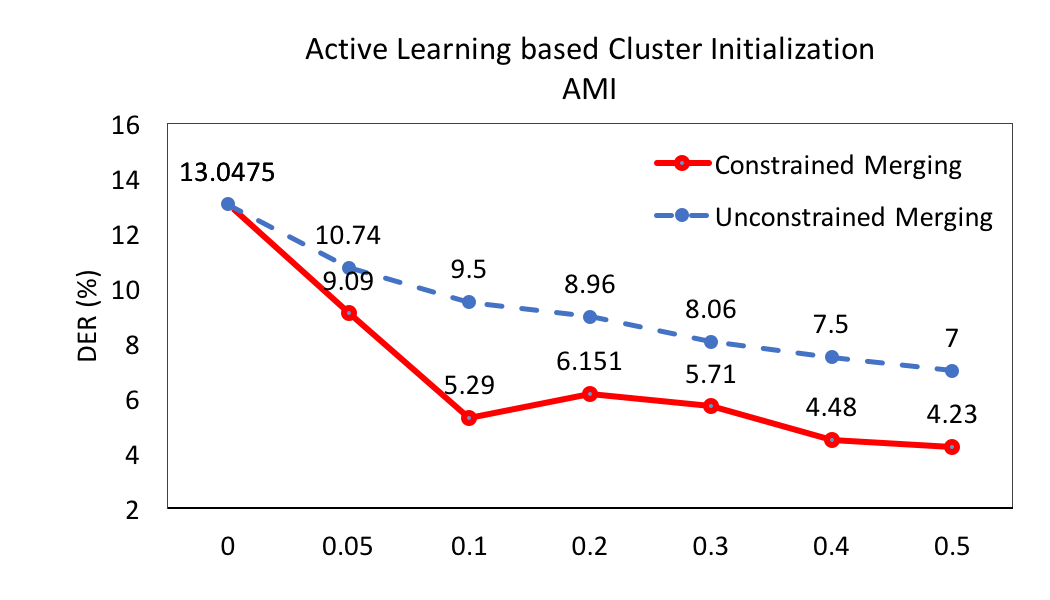
\includegraphics[width=\linewidth]{figs/exp1_1}
	\caption{Results of proposed active learning based speaker clustering algorithm on AMI meeting corpus. The red line is the diarization error rate (DER) with constrained clustering, while the blue dotted line is result obtained with unconstrained clustering as in baseline speaker clustering algorithms. Both constrained and unconstrained clustering performed after \textit{explore} stage. The horizontal axis is the amount of query pairs proportional to total number of speech segments $N$. }
	\label{exp1_1}
\end{figure}
\begin{figure}[t]
	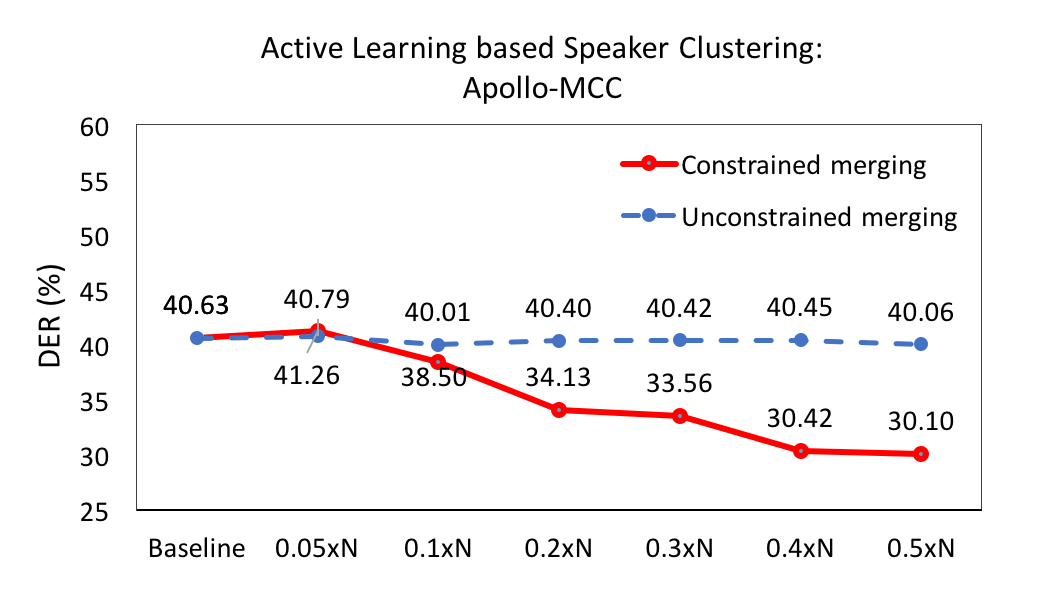
\includegraphics[width=\linewidth]{figs/exp1_2}
	\caption{Results of proposed active learning based speaker clustering algorithm on Apollo Mission Control Center (Apollo-MCC) audio dataset. The red line is the diarization error rate (DER) with constrained clustering, while the blue dotted line is result obtained with unconstrained clustering as in baseline speaker clustering algorithms. Both constrained and unconstrained clustering performed after \textit{explore} stage. The horizontal axis is the amount of query pairs proportional to total number of speech segments $N$.}
	\label{exp1_2}
\end{figure}
\begin{table}[]
	\centering
	\caption{Evaluation of different query selection algorithm in \textit{explore} stage using AMI dataset.}
	\label{ffqs}
	\begin{tabular}{@{}lccc@{}}
		\toprule
		& explore (0.05xN)  & explore (0.1xN)  & explore (0.2xN)   \\ \midrule
		Baseline            & 13.04 & 5.29 & 13.04 \\ \midrule
		Random Selection    & 9.05  & 6.08 & 6.17  \\ \midrule
		FFQS (random seed)  & 9.12  & 6.17 & 6.02  \\ \midrule
		FFQS (cluster seed) & 9.09  & 5.29 & 6.15  \\ \bottomrule
	\end{tabular}
\end{table}
\begin{figure}
	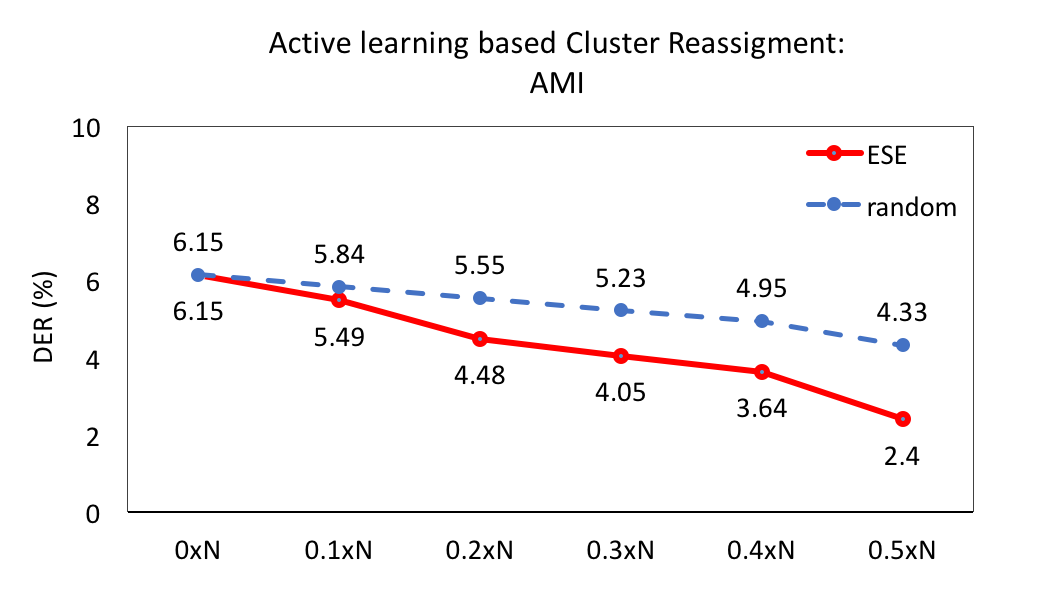
\includegraphics[width=\linewidth]{figs/exp2_2}
	\caption{Results of proposed active learning based cluster reassignment algorithm on AMI meeting corpus. The red line is the diarization error rate (DER) using the expected speaker error (ESE) as criteria for candidates selection, while the blue dotted line is DER obtained by randomly selecting segments as candidates for evaluation and reassignment. The horizontal axis is the amount of candidate segments proportional to total number of speech segments $N$.}
	\label{exp2_1}
\end{figure}
\begin{figure}
	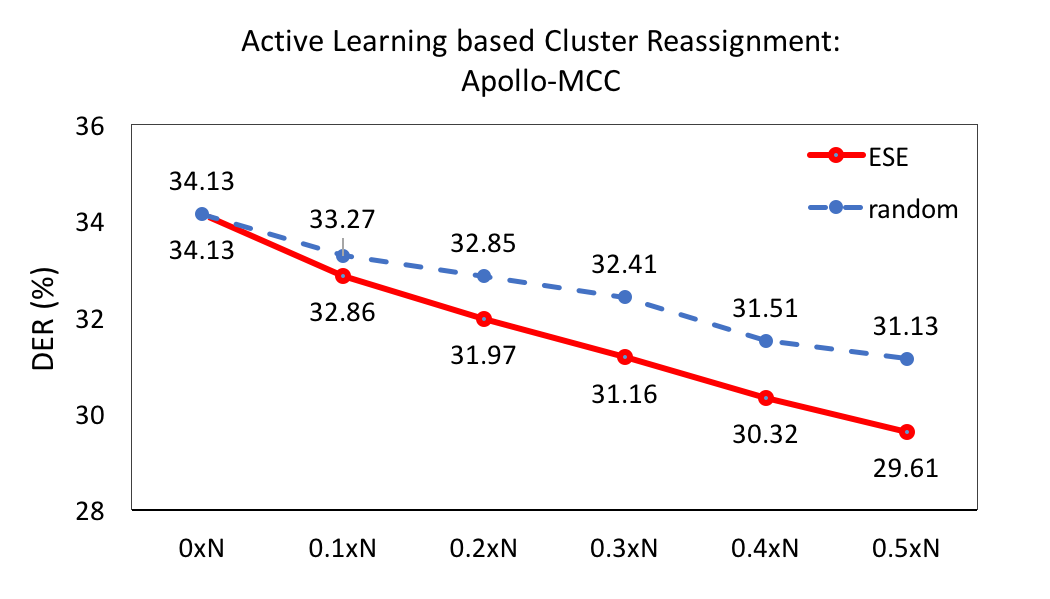
\includegraphics[width=\linewidth]{figs/exp2_1}
	\caption{Results of proposed active learning based cluster reassignment algorithm on Apollo Mission Control Center (Apollo-MCC) corpus. The red line is the diarization error rate (DER) using the expected speaker error (ESE) as criteria for candidates selection, while the blue dotted line is DER obtained by randomly selecting segments as candidates for evaluation and reassignment. The horizontal axis is the amount of candidate segments proportional to total number of speech segments $N$.}
	\label{exp2_2}
\end{figure}

\subsection{Active Learning Based Speaker Clustering}
In this experiments, we evaluate the performance of active learning based speaker clustering, by varying the amount of human effort in terms of number of queries. Note that, the total number of queries to achieve perfect clustering result is $\dfrac{N(N-1)}{2}$ , where $N$ is total segment in test audio.
For all our experiments in this study, we will access to the reference answers of questioned pair, assuming no errors from human experts. However, in future study, it will be necessary to consider the human errors into account.

We will evaluate the proposed algorithm by varying the quantify of the pairs as a function of total segment number of $N$. For example, if a test audio stream has 1000 speech segments, active learning $0.1\cdot N$ query pairs means we have access to 100 query pairs out of $1000*(1000-1)/2$ total pairs. If we assume each speech segments has an average length of 2 seconds, the evaluation of 100 query pairs will spend about 400 (100*2*2) seconds for human evaluation. This is very small amount of human evaluation time compared to the total time requires human to obtain perfect speaker diarization which is ($1000*(1000-1)/2*2*2$) in the worst case in the example.

The red line in Figure.~\ref{exp1_1} and Figure.~\ref{exp1_2} shows the performance of proposed active learning based speaker clustering algorithm with varying amount of human input. The result with zero queries $0$x$N$, indicates results from baseline bottom-up speaker diarization algorithm. The first thing we notice is that the baseline DER in Apollo-MCC (40.63\%) is much higher than that of AMI dataset (10.83\%). Such difference in performances are expected due to the challenges within Apollo-MCC dataset we illustrated in Section.~\ref{apollo}. We could also see from the results, DER reduce rapidly with relatively small amount of human input. In case of AMI dataset, the DER reduce from 10.83\% to 9.09\%, a relative of 16\% reduction with only $0.05$x$N$ query pairs, and this number further reduce to 5.29\% with $0.1$x$N$ queries. In case of Apollo-MCC dataset, the proposed algorithm is also capable of effectively reducing the DER, although it requires much more human input compared with AMI dataset. This might attributes to the significantly larger participants within Apollo-MCC dataset, which requires more human input during \textit{explore} stage, to discover all involved speakers. 

\begin{figure*}[t]
	\centering
	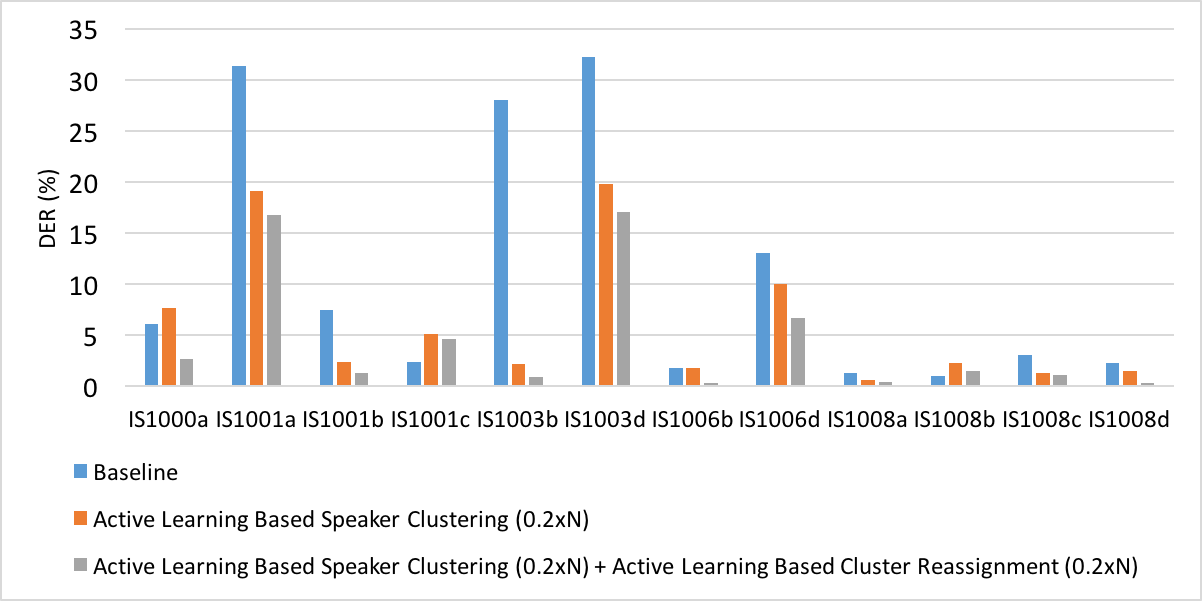
\includegraphics[width=0.75\linewidth]{figs/exp3_1}
	\caption{Results of proposed active learning based cluster reassignment algorithm on AMI meeting corpus. The red line is the diarization error rate (DER) using the expected speaker error (ESE) as criteria for candidates selection, while the blue dotted line is DER obtained by randomly selecting segments as candidates for evaluation and reassignment. The horizontal axis is the amount of candidate segments proportional to total number of speech segments $N$.}
	\label{exp2_1}
\end{figure*}

\subsubsection{Importance of \textit{constrained clustering}}
We also evaluate the importance of \textit{constrained clustering} in active learning based speaker clustering. The blue dotted lines in Figure.~\ref{exp1_1} and Figure.~\ref{exp1_2} indicates the performance using traditional bottom-up clustering without any constraint in merging, after \textit{explore} stage. And red dotted lines n Figure.~\ref{exp1_1} and Figure.~\ref{exp1_2} shows the performance with \textit{constrained clustering} where bottom-up clustering is performed with a constraint that the clusters created in \textit{explore} stage can not merge with each other. Comparing these two results, we could see that it is extremely important to perform \textit{constrained clustering}. Only small improvement in AMI dataset and nearly no improvements in speaker diarization is observed if without using \textit{constrained clustering}. This indicates that our proposed active learning based speaker diarization is essentially transforms unsupervised speaker diarization task into something similar to supervised close-set speaker identification tasks, and therefore be able to achieve significant improvements.

\subsubsection{FFQS in \textit{explore} stage}
In this experiments, we evaluate farthest first query search (FFQS) strategy used in \textit{explore} stage. There are two alternative FFQS, depending on how to select initial seed. We also compare FFQS performance with random selection, where the query selection is based on complete randomness. The results are listed in Table.~\ref{ffqs}. The results obtained with random selection and FFQS based on random seeding both involves the randomness, thus the obtained results are an average of 10 different experiments. We could see from the results that, the average performance does not vary to much on the algorithm used during \textit{explore} stage. However, we observe large variance in the performances of random selection and FFQS with random seed, therefore we conclude that the FFQS with initial seeds obtaining from centroids of unsupervised clustering results are more preferable.

\subsubsection{limitations}
While the experiment results in Figure.~\ref{exp1_1} and Figure.~\ref{exp1_2} has shown that proposed active learning based speaker clustering algorithm drops the DER quickly with relatively small amount of human input, the performance saturates as more human input are provided. This is expected behavior, as the objective of proposed algorithm is to discover all involved speakers, and initialize reliable initial speaker models for each of them. As long as the majority of speakers are discovered with relative sufficient number of instances, the benefit of using more human input will be inconsequential. This poses a limitation in certain scenarios, where human input are needed to further drops the DER.

\subsection{Active Learning Based Cluster Reassignment}
In this experiment, we continue to improve speaker diarization performance using our second active learning algorithm: active learning based cluster reassignment. For both experiments on Apollo-MCC audio dataset and AMI meeting corpus, we use at most 10 instances per cluster, to compose query pairs for majority voting based evaluation of whether a particular segment belongs to target cluster. We also fix our n-best search to the rank of 3, during the search of correct cluster assignment. We evaluate our active learning algorithm by varying the amount of we will select for evaluation and reassignment. We also define this amount with respect to total number of segments $N$. For example, if the total number of speech segments in an audio stream is $N=1000$,  evaluation of $0.1$x$N$ segments means human expert will review 100 speech segments, which requires access to 100*3*10 queries with correct answer if we uses n-best rank of 3, and 10 instances per cluster.

The red lines in Figure.~\ref{exp2_1} and Figure.~\ref{exp2_2} indicates the performance of proposed active learning based speaker clustering algorithm on AMI and Apollo-MCC dataset, respectively. We uses clustering output from active learning based speaker clustering algorithm ($0.2$x$N$ condition) as a base for performing cluster reassignment. We could see that the DER drops consistently as more segments are selected for reassignments. In case of AMI dataset, the DER reduce from 6.15\% to 5.49\%, a relative of 10\% reduction with only $0.1$x$N$ query pairs, and this number continue to reduce as more segments are selected for reassignment. The similar trend is also observed in the results from Apollo-MCC dataset, although the relative improvement in Apollo-MCC relative smaller than that in AMI dataset.

\subsubsection{Expected speaker error based candidate selection}
In this section, we evaluate the effectiveness of using expected speaker error (ESE) as criteria for selecting segment candidates for human reassignment. We compare largest ESE based candidate selection with random segment selection. The red lines in Figure.~\ref{exp2_1} and Figure.~\ref{exp2_2} indicates the performance of using ESE as criteria, while the blue dotted line in Figure.~\ref{exp2_1} and Figure.~\ref{exp2_2} indicates the performance of random segment selection. The results clearly shows that the DER drops much faster with ESE based candidate selections, in both AMI and Apollo dataset.

\section{Conclusion}

\section*{Acknowledgments}
This research was supported by National Science Foundation (NSF) under Grant 1219130.
 


%\appendices
%\section{Proof of the First Zonklar Equation}
%Appendix one text goes here.

% you can choose not to have a title for an appendix
% if you want by leaving the argument blank
%\section{}
%Appendix two text goes here.

% use section* for acknowledgement
%\section*{Acknowledgment}

%The authors would like to thank...

% Can use something like this to put references on a page
% by themselves when using endfloat and the captionsoff option.
\ifCLASSOPTIONcaptionsoff
  \newpage
\fi

\bibliographystyle{IEEEtran}
\bibliography{IEEEabrv,MOREabrv,strings,ref}


\end{document}


